\section{D-RI5CY -- Vulnerability Assessment}

%%%%%%%%%%%%%%%%%%%%%%%%%%%%%%%%%%%%%%%%%%%%%%%%%%%%%%%%%%%%%%%%%%%%%%%%%%%%
\subsection{D-RI5CY - origins and architecture}
\begin{frame}{D-RI5CY - origins}
    \begin{itemize}
        \item Design~\cite{PDGLC-18-hpec} made by researchers at Columbia University (USA) with Politecnico di Torino (Italy)
        \item Based on the 32-bit RISC-V processor: RI5CY (Pulp Platform)
        \item Open source\footnote{\url{https://github.com/sld-columbia/riscv-dift}}
        \item 1-bit tag datapath
        \item Flexible security policy that can be modified at runtime
    \end{itemize}

    \centering
    \vfill
    
\includegraphics[height=1cm]{img/logo/riscv.png}
    \hspace{1cm}
    
\includegraphics[height=1cm]{img/logo/pulp_logo.pdf}
    \vfill
\end{frame}
%%%%%%%%%%%%%%%%%%%%%%%%%%%%%%%%%%%%%%%%%%%%%%%%%%%%%%%%%%%%%%%%%%%%%%%%%%%%
\begin{frame}{D-RI5CY - architecture}
    \begin{figure}
        \centering
        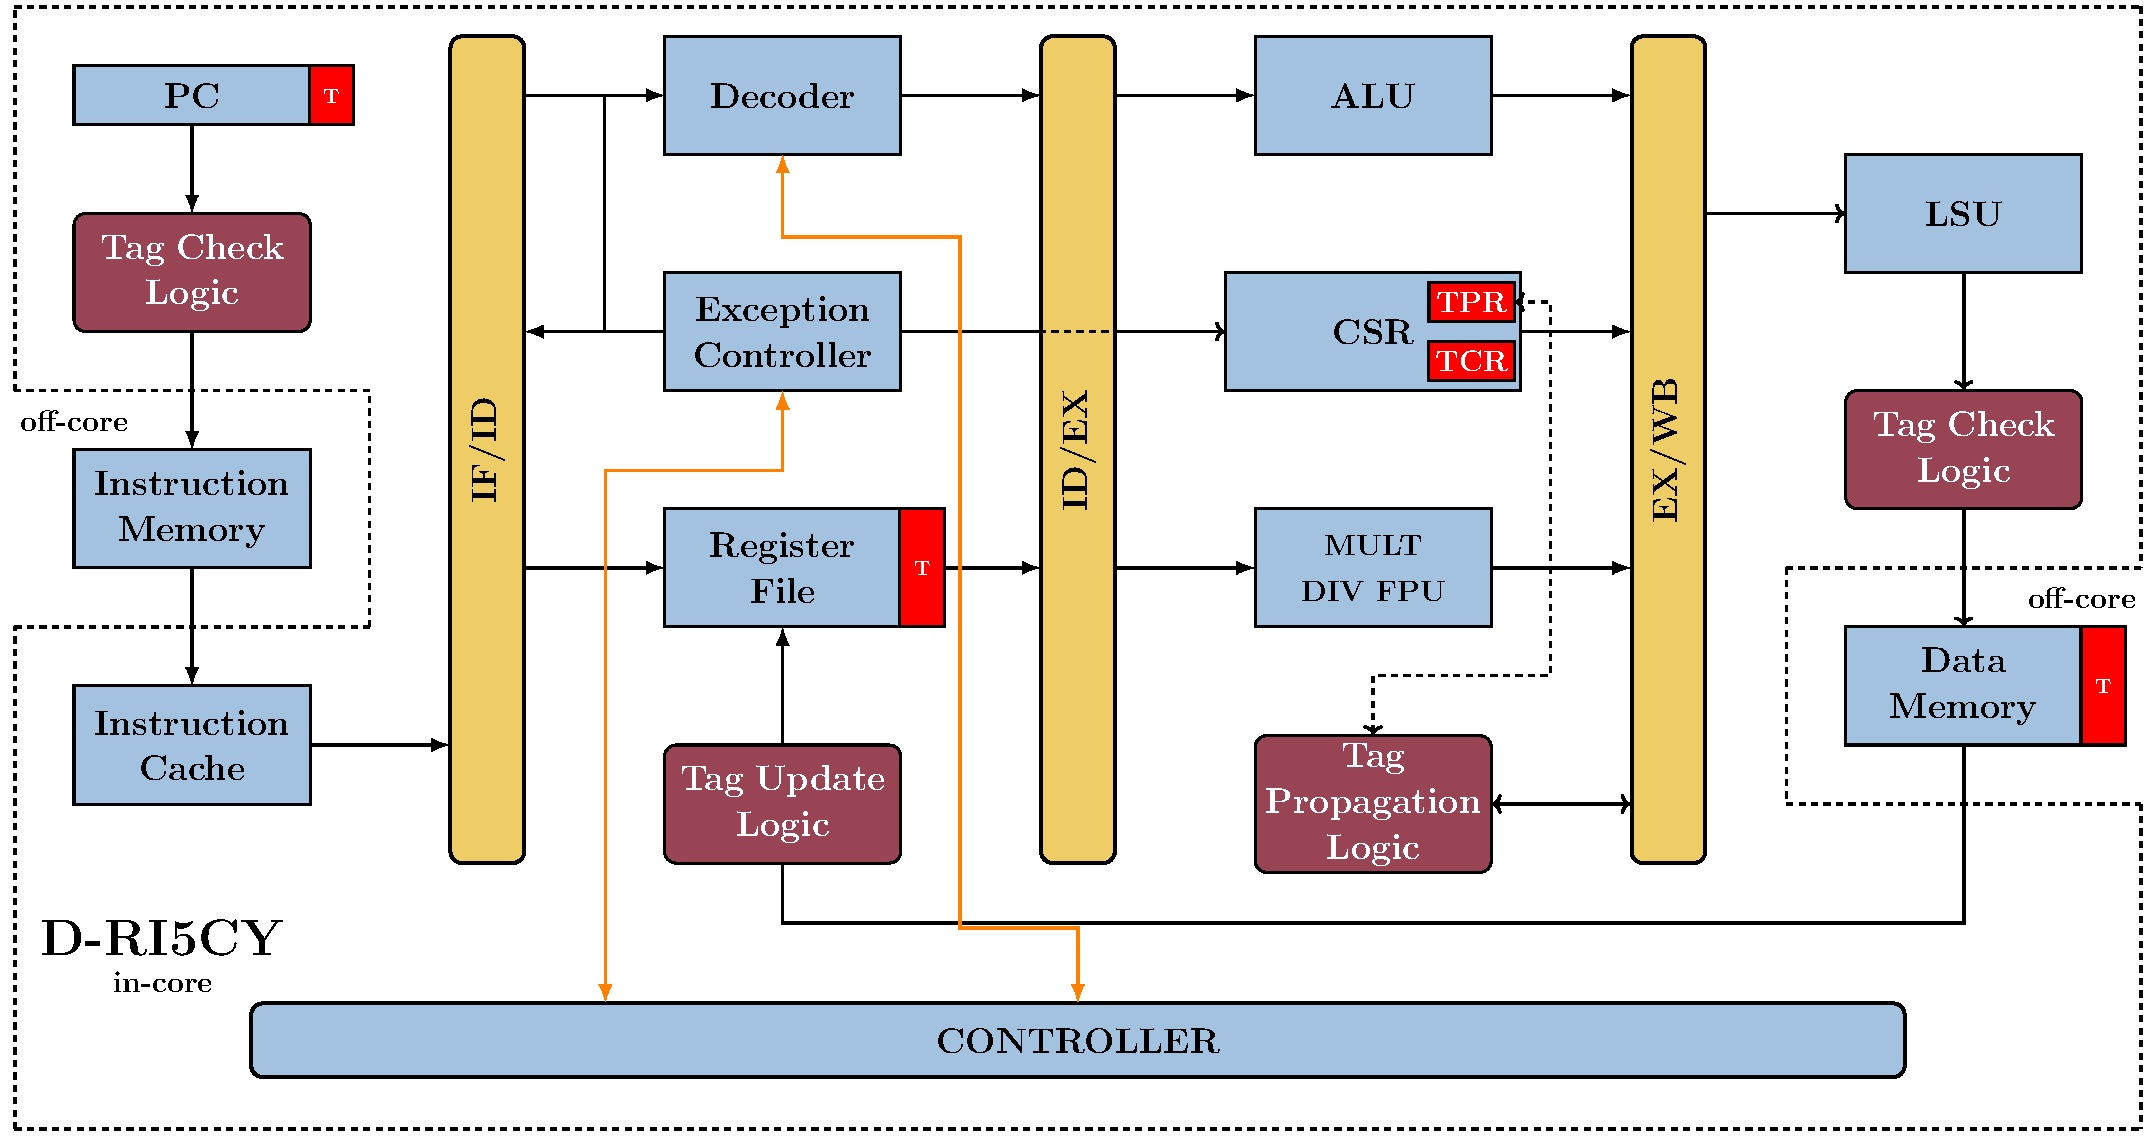
\includegraphics[width=.9\textwidth]{src/2_vuln_assessment/img/RI5CY.pdf}
        \caption{Architecture of the D-RI5CY.}
        \label{fig:riscy}
    \end{figure}
\end{frame}
%%%%%%%%%%%%%%%%%%%%%%%%%%%%%%%%%%%%%%%%%%%%%%%%%%%%%%%%%%%%%%%%%%%%%%%%%%%%
\subsection{Vulnerability assessment}
\begin{frame}{Vulnerability Assessment}
    \begin{block}{Threat model}
        We consider an attacker able to:
        \begin{itemize}
            \item perform a physical attack to defeat the DIFT mechanism and realise a software attack,
            \item inject faults in DIFT-related registers:
                  \begin{itemize}
                      \item bit set,
                      \item bit reset,
                      \item bit-flip.
                  \end{itemize}
        \end{itemize}
    \end{block}

    % \begin{block}{Methodology}
    %     \begin{itemize}
    %         \item Analysis of 2 attacks use cases: buffer overflow attack, format string attack
    %         \item Analysis of 1 use case to cover the DIFT surface: compare/compute
    %     \end{itemize}
    % \end{block}
\end{frame}
%%%%%%%%%%%%%%%%%%%%%%%%%%%%%%%%%%%%%%%%%%%%%%%%%%%%%%%%%%%%%%%%%%%%%%%%%%%%
\subsection{Use case : presentation}
\begin{frame}{Case 1: Buffer overflow}
    \begin{itemize}
        \item The attacker exploits a buffer overflow to access the return address register ($RA$).
    \end{itemize}

    \begin{figure}
        \centering
        \begin{subfigure}[l]{.45\textwidth}
            \centering
            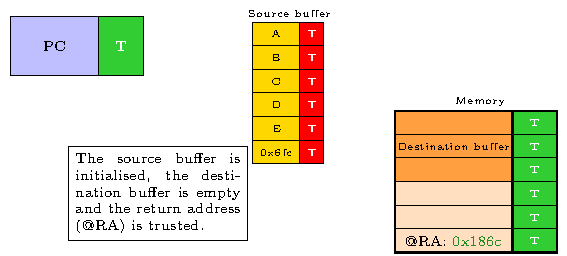
\includegraphics[width=.9\textwidth, page=1]{src/2_vuln_assessment/img/buffer_overflow/schemaPedagogique.pdf}
            \caption{Malicious buffer and $RA$ trusted}
            \label{fig:bo_1st_step}
        \end{subfigure}
        \begin{subfigure}[r]{.45\textwidth}
            \centering
            \includegraphics[width=.9\textwidth, page=5]{src/2_vuln_assessment/img/buffer_overflow/schemaPedagogique.pdf}
            \caption{Overflow and overwriting of $RA$ and its tag}
            \label{fig:bo_3rd_step}
        \end{subfigure}
    \end{figure}

    \begin{itemize}
        \item As the data in the source buffer is manipulated by the user, it is marked as \textcolor{red}{\textit{untrusted}}.
        \item Thanks to DIFT, the tags associated with the source buffer data overwrite the $RA$ register tag.
        \item When the function returns, the corrupted register $RA$ is loaded into $PC$ using a jalr instruction.
    \end{itemize}
\end{frame}

\begin{frame}
    \begin{figure}
        \centering
        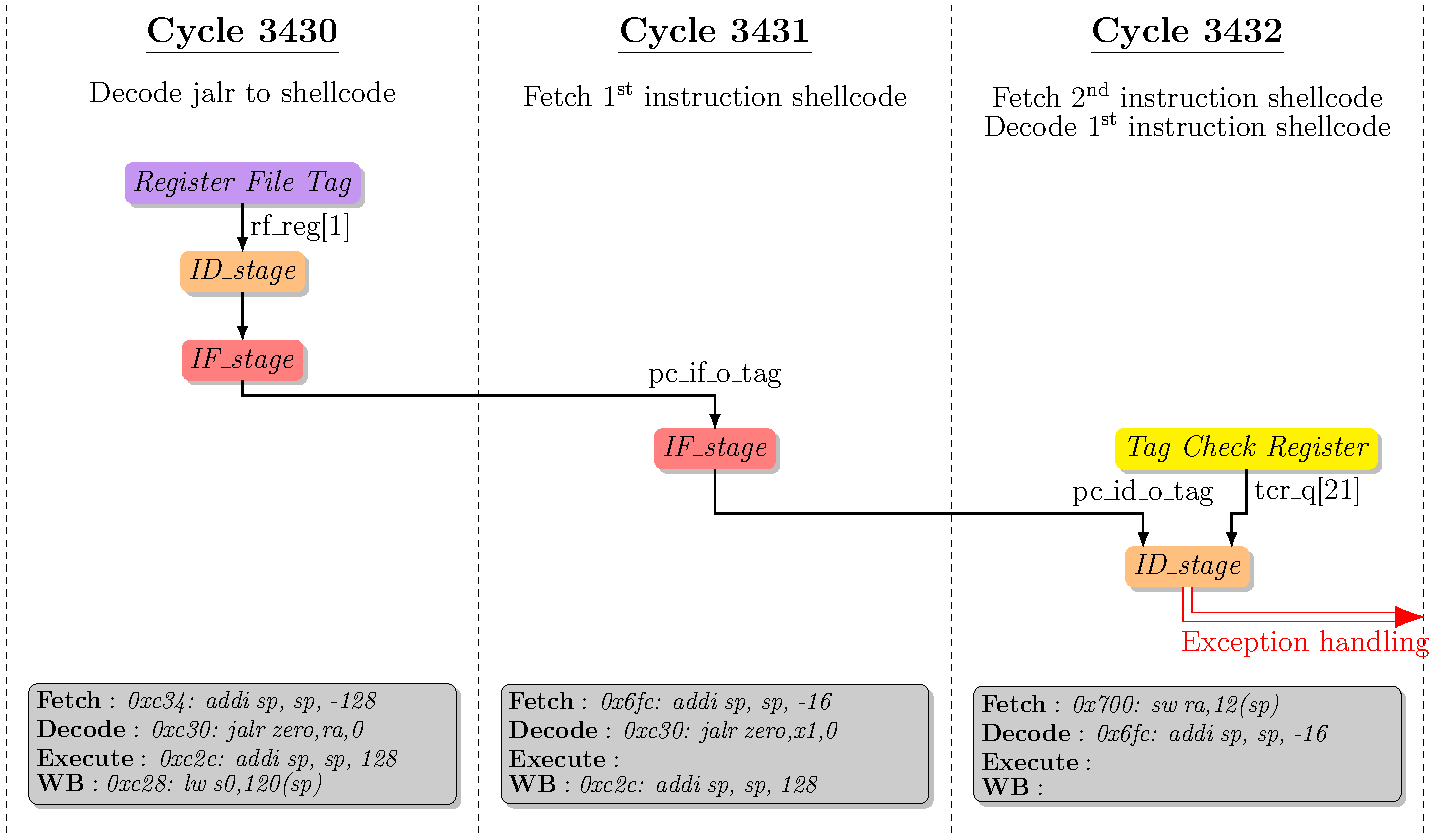
\includegraphics[width=.75\textwidth]{src/2_vuln_assessment/img/buffer_overflow/bufferOverflowAttack_short.pdf}
        \caption{Temporal analysis of the tags propagation in \textit{Buffer Overflow} attack}
        \label{fig:analyseTempoBufferOverflow}
    \end{figure}
\end{frame}

\begin{frame}
    \begin{figure}
        \centering
        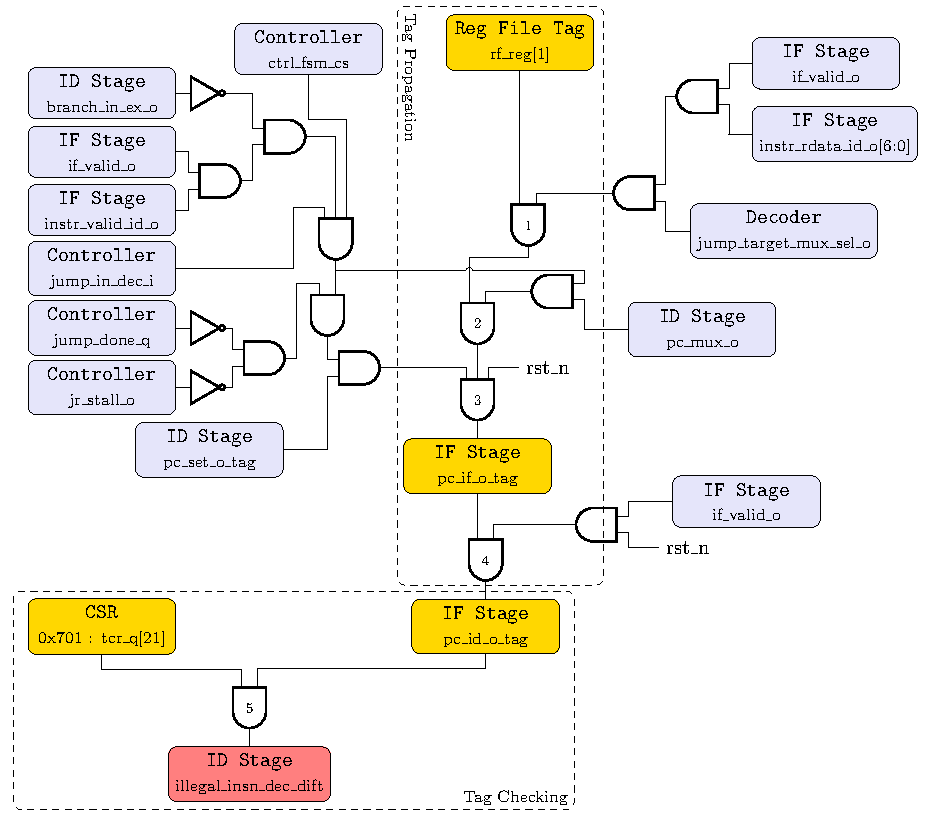
\includegraphics[height=.85\textheight]{src/2_vuln_assessment/img/buffer_overflow/arborescence_bufferOverflow.pdf}
        \caption{Logical analysis of the tags propagation in a \textit{Buffer Overflow} attack}
        \label{fig:analyseLogiqueBufferOverflow}
    \end{figure}
\end{frame}
%%%%%%%%%%%%%%%%%%%%%%%%%%%%%%%%%%%%%%%%%%%%%%%%%%%%%%%%%%%%%%%%%%%%%%%%%%%%%%%%%%%%%%%%%%%%%%%%%%%%%%%%%%%%
\subsection{Experimental Setup}
%%%%%%%%%%%%%%%%%%%%%%%%%%%%%%%%%%%%%%%%%%%%%%%%%%%%%%%%%%%%%%%%%%%%%%%%%%%%%%%%%%%%%%%%%%%%%%%%%%%%%%%%%%%%
\begin{frame}{Experimental Setup - Simulation fault injections campaign}
    \begin{itemize}
        \justifying
        \item Logical fault injection simulation is used for preliminary evaluations
              \begin{itemize}
                  \justifying
                  \item faults are injected in the HDL code at cycle accurate and bit accurate level
                  \item a set of 55 DIFT-related registers are targeted
                  \item a reference simulation is done without fault
                  \item results are classed in four groups
                        \begin{itemize}
                            \justifying
                            \item crash: reference cycle count exceeded,
                            \item silent: current faulted simulation is the same as the reference simulation
                            \item delay: illegal instruction is delayed
                            \item success: DIFT has been bypassed
                        \end{itemize}
              \end{itemize}
        \item Simulations with QuestaSim 10.6e.
        \item FISSA is used in order to create our injection campaigns
    \end{itemize}
\end{frame}
%%%%%%%%%%%%%%%%%%%%%%%%%%%%%%%%%%%%%%%%%%%%%%%%%%%%%%%%%%%%%%%%%%%%%%%%%%%%%%%%%%%%%%%%%%%%%%%%%%%%%%%%%%%%
\begin{frame}{Main results : 3 cases}
    \begin{table}[H]
        \centering
        \caption{End of simulation status}
        \label{table:end_sim_by_status}
        \begin{tabular}{lrrrlr}
            \toprule
                            & Crash & NSTR & Delay & Success     & Total \\
            \midrule
            Buffer overflow & 0     & 1380 & 20    & 24 (1.69\%) & 1422  \\
            WU-FTPd         & 0     & 1767 & 77    & 52 (2.74\%) & 1896  \\
            Compare/Compute & 0     & 917  & 12    & 19 (2.00\%) & 948   \\
            \bottomrule
        \end{tabular}
    \end{table}
\end{frame}

\begin{frame}{Buffer overflow}
    \begin{table}[]
        \centering
        \caption{Buffer overflow : Register sensitivity as determined by fault model and simulation time}
        \label{table:end_sim_from_time_fault_register_buffer_overflow}
        \resizebox{\textwidth}{!}{%
            \begin{tabular}{llllllllllllllll}
                \toprule
                                                & \multicolumn{3}{c}{Cycle 3428} & \multicolumn{3}{c}{Cycle 3429} & \multicolumn{3}{c}{Cycle 3430} & \multicolumn{3}{c}{Cycle 3431} & \multicolumn{3}{c}{Cycle 3432}                                                                                                                 \\\cmidrule(lr){2-4}\cmidrule(lr){5-7}\cmidrule(lr){8-10}\cmidrule(lr){11-13}\cmidrule(lr){14-16}
                                                & set0                           & set1                           & bitflip                        & set0                           & set1                           & bitflip    & set0       & set1 & bitflip    & set0       & set1 & bitflip    & set0       & set1 & bitflip    \\
                \midrule
                pc\_if\_o\_tag                  &                                &                                &                                &                                &                                &            &            &      &            & \checkmark &      & \checkmark &            &      &            \\
                memory\_set\_o\_tag             &                                & \checkmark                     & \checkmark                     &                                &                                &            &            &      &            &            &      &            &            &      &            \\
                rf\_reg[1]                      &                                &                                &                                &                                &                                &            & \checkmark &      & \checkmark &            &      &            &            &      &            \\
                tcr\_q                          & \checkmark                     &                                &                                & \checkmark                     &                                &            & \checkmark &      &            & \checkmark &      &            & \checkmark &      &            \\
                \rowcolor{LightGray} tcr\_q[21] &                                &                                & \checkmark                     &                                &                                & \checkmark &            &      & \checkmark &            &      & \checkmark &            &      & \checkmark \\
                tpr\_q                          & \checkmark                     & \checkmark                     &                                & \checkmark                     & \checkmark                     &            &            &      &            &            &      &            &            &      &            \\
                \rowcolor{LightGray} tpr\_q[12] &                                &                                & \checkmark                     &                                &                                & \checkmark &            &      &            &            &      &            &            &      &            \\
                \rowcolor{LightGray} tpr\_q[15] &                                &                                & \checkmark                     &                                &                                & \checkmark &            &      &            &            &      &            &            &      &            \\
                \bottomrule
            \end{tabular}
        }
    \end{table}
\end{frame}

\begin{frame}{Discussion}
    \begin{itemize}
        \setbeamertemplate{itemize items}[triangle]
        \item 4266 simulations have been performed,
        \item 95 successes (2.23\%),
        \item We have shown that the D-RI5CY DIFT is vulnerable to FIA
        \item Propagation of faults is facilitated by paths fully made of \textit{AND} gates
    \end{itemize}
\end{frame}
%%%%%%%%%%%%%%%%%%%%%%%%%%%%%%%%%%%%%%%%%%%%%%%%%%%%%%%%%%%%%%%%%%%%%%%%%%%%%%%%%%%%%%%%%%%%%%%%%%%%%%%%%%%%